%Triangulo de pascal
\newlength{\R}
\setlength{\R}{.75cm}
\newcommand\mycolor{white}

%% https://tex.stackexchange.com/questions/34424/how-do-i-calculate-n-modulo-3-in-latex/34425#34425
\newcommand{\modulo}[2]{%
  \FPeval{\result}{trunc(#1-(#2*trunc(#1/#2,0)),0)}\result%
}

%%  #1 determines which hexagons are filled (default is 2); #2 is number of rows

\newcommand{\makesierp}[2][2]{%
    \begin{tikzpicture}[line width=.8pt]
        \foreach \k in {0,...,#2}{
            \begin{scope}[shift={(-60:{sqrt(3)*\R*\k})}]
                \pgfmathtruncatemacro\ystart{#2-\k}
                \foreach \n in {0,...,\ystart}{
                    \pgfmathtruncatemacro\newn{\n+\k}
                    \pgfmathsetmacro{\myvalue}{1}
                    \ifnum\k>0
                        \foreach \b in {1,...,\k}{
                            \FPeval\myvalue{trunc(\myvalue*(\newn-\b+1)/\b:0)}
                            \global\let\myvalue=\myvalue
                        }
                    \fi
                    \modulo{\myvalue}{#1}%
                    \ifnum\result=0 \def\mycolor{green}\fi%
                    \begin{scope}[shift={(-120:{sqrt(3)*\R*\n})}]
                        \draw[fill=\mycolor!20] 
                        (30:\R) \foreach \x in {90,150,...,330} {
                        -- (\x:\R)}
                        --cycle (90:0)node[font=\tiny] {$\mathbf{\myvalue}$};
                    \end{scope}
                }
            \end{scope}
        }
    \end{tikzpicture}
}

\textbf{Definition of Pascal's Triangle} \\
Pascal's Triangle is a mathematical construct that is used in various areas of mathematics, particularly in combinatorics and algebra. It is a triangular array of numbers in which each number is the sum of the two numbers directly above it. The triangle is named after the French mathematician Blaise Pascal, who studied its properties in the 17th century, although it was known to Chinese mathematicians over 500 years earlier.  \\

Pascal's Triangle is an infinite triangular array of numbers in which the first and last numbers in each row are always 1, and each of the interior numbers is the sum of the two numbers directly above it.  \\

%Triangulo de pascal
\resizebox{0.8\textwidth}{!}{ 
    \makesierp{20}
}
 %INSERTAR

\vspace{1cm}
\noindent \textbf{Applications of Pascal Triangle}
Pascal's Triangle, a mathematical construct developed by Blaise Pascal, has several applications in the field of biology. Here are some of the uses of Pascal's Triangle in biology:  \\

\noindent 1. Genetic Inheritance: Pascal's Triangle can be used to understand and calculate the probabilities of different genetic inheritance patterns. For example, it can help determine the probability of specific genotypes or phenotypes in offspring when considering traits governed by multiple alleles or multiple genes. \\

\noindent 2. Population Genetics: In the study of population genetics, Pascal's Triangle can be employed to model changes in allele frequencies over time. It aids in predicting the distribution of genotypes within a population across generations, considering factors like genetic drift, mutation rates, and selection pressures. \\

\noindent 3. Probability in Genetics: Pascal's Triangle is useful for calculating probabilities in genetic crosses involving complex inheritance patterns. It can help determine the likelihood of certain genetic outcomes in offspring, which is essential for understanding the genetic basis of traits and diseases. \\

\noindent 4. Microbial Population Growth: In microbiology, Pascal's Triangle can be applied to model the growth of microbial populations. It helps researchers predict population sizes over time under various conditions, such as different growth rates and mutation rates. \\

\noindent 5. Evolutionary Biology: Pascal's Triangle can be used to analyze the probabilities of specific genetic changes occurring over time within populations. This is crucial for studying the emergence of new traits and adaptations during evolution. \\

\noindent 6. Phylogenetics: In phylogenetics, which focuses on the evolutionary relationships among species, Pascal's Triangle can be used to calculate the probabilities of different phylogenetic tree topologies based on genetic data. It aids in inferring the evolutionary history and relationships of species. \\

\noindent 7. Population Ecology: Pascal's Triangle can be employed in population ecology to model changes in population size over time. It helps predict how populations of different species interact within ecological communities and how they respond to changes in birth rates, death rates, immigration, and emigration. \\

\noindent 8. Epidemiology: In epidemiology, Pascal's Triangle can be used to model the spread of diseases within populations. It aids in understanding the probabilities of individuals becoming infected, recovering from infections, or transmitting diseases to others. This is valuable for disease control and public health efforts. \\

\noindent 9. Genetic Mapping: Pascal's Triangle can assist in genetic mapping by           calculating probabilities related to the linkage of genetic markers on chromosomes. It helps determine the likelihood of two or more genes segregating together or independently during meiosis. \\

\noindent 10. Probability of Mutations: Researchers can use Pascal's Triangle to calculate the probabilities of specific types of mutations occurring in DNA sequences. This is crucial for understanding the molecular basis of genetic diseases and evolutionary processes. \\

\textbf{Example: GENETICS}

Pascal's Triangle and Risk Calculations \\
Introduction: \\
Pascal's Triangle, based upon the French Mathematician Blaise Pascal, is used in genetic counselling to calculate the probability of obtaining a particular number or distribution of events of one kind knowing the probability of each event occurring independently. This is a simpler approach to the use of the Binomial Distribution. \\

Principles: Pascal's Triangle \\
The simplest way to look at the role of Pascal's Triangle is to study a family with an autosomally inherited disorder. \\
What are Autosomes? \\
Autosomes are non-sex chromosomes found in the cells of an organism. In humans and many other organisms, autosomes make up the majority of an individual's total chromosome number. They are distinct from the sex chromosomes (X and Y in humans) that determine an individual's sex. Autosomes carry genes responsible for various traits and characteristics unrelated to sexual development.
Consider the following scenario: \\
A 45-year-old man is diagnosed with Type 1 Antithrombin deficiency and is concerned that he may have passed it onto his three children. His partner has normal functional Antithrombin levels. what are the risk that his children will have Type 1 Antithrombin deficiency. \\
Antithrombin deficiency is inherited as an autosomal dominant disorder. \\

\textbf{Example: GENETICS}
The Family Pedigree is shown below: \\

\begin{figure}
    \centering
    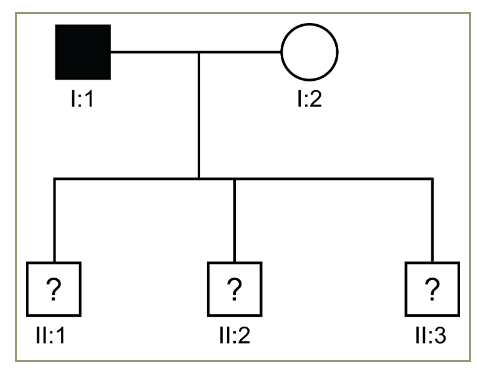
\includegraphics[width=0.5\linewidth]{1 Introducción/Tareas Capítulo 1/Triángulo de Pascal/Picture2.png}
    \caption{Example: GENETICS}
    \label{fig:enter-label}
\end{figure}

\textbf{What are the Risks?} \\
1. All 3 of his children [II:1, II:2 and II:3] will have Type 1 Antithrombin deficiency? \\

2. All 3 of his children [II:1, II:2 and II:3] will not have Type 1 Antithrombin deficiency? \\

3. 1 of his children will have Type 1 Antithrombin deficiency? \\

4. 2 of his children will have Type 1 Antithrombin deficiency? \\

We can derive the answers for these questions using Pascal's Triangle - derived by expanding (p +q)n. This is shown diagrammatically below: \\

\begin{figure}
    \centering
    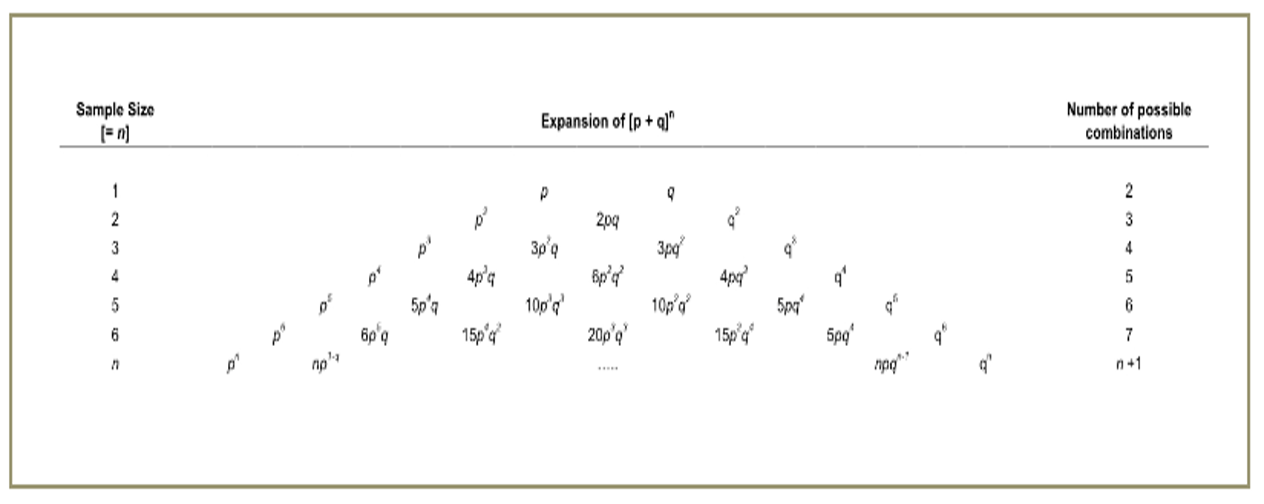
\includegraphics[width=1\linewidth]{1 Introducción/Tareas Capítulo 1/Triángulo de Pascal/Picture3.png}
    \caption{Example: GENETICS}
    \label{fig:enter-label}
\end{figure}

\noindent So - if we look at the family with 3 possible children [n = 3] and if read along the Triangle, we see that for all 3 of the children to have Type I Antithrombin deficiency the probability is [q]3 where q = 1/2 and so [1/2]3 = 1/8. \\
\noindent Antithrombin deficiency is an autosomally inherited disorder and the risk of inheriting a mutant allele from a parent is 1/2 and of not inheriting it, is also 1/2.   So the probability that all 3 children will be normal [p]3 is 1/8 and similarly the probability that all 3 children will have Type 1 Antithrombin deficiency, is [q]3 which is also 1/8. \\
To establish if only 1 of the children will be affected and the other two normal then again we read along from n=3 to where we see 3pq2 and so 3pq2 = 3 x 1/2 x [1/2]2 = 3 x 1/2 x 1/4 = 3/8. So the risk that they will have one affected child and two normal children is 3/8.
\noindent Remember p is the probability of an event not occurring - in this case not inheriting the disorder and q is the probability of an event occurring - in this case inheriting the disorder \\

\noindent Podemos construir el triangulo en python tambien, de la siguiente manera. \\

\begin{verbatim}
    # Doing the Pascal's Triangle using Python
    def factorial(num):
        if num > 0:
            # Doing the factorial using recursion
            return int(num*factorial(num-1))
        else:
            return 1
    
    def combinatoria(num1, num2):
        return int(factorial(num1) / (factorial(num2)*factorial(num1-num2)))
    
    def crearTriangulo(n_filas):
        for fila in range(n_filas):
            for j in range(n_filas-fila+1):
                print(" ", end="")
            if fila == 0:
                print("1 1")
            else:
                for j in range(fila+2):
                    print(combinatoria(fila+1, j), end=" ")
                print()
    
    crearTriangulo(int(input("Indica el número de filas que desee: ")))
    
\end{verbatim}

\noindent O en C++, utilizando en siguiente codigo:\\

\begin{verbatim}
    #include<iostream>
    
    long factorial(int x){
    	if(x > 0){
    		return x * factorial(x-1); //Recursividad
    	}else{
    		return 1;
    	}
    }
    int combinatoria(int num1, int num2){
    	return ((int) factorial(num1))/ (factorial(num2)*factorial(num1-num2));
    }
    void imprimirTriangulo(int filas){
    	for(int i=1;i<=filas;i++){
    		for(int j=0;j<(filas-i);j++){
    			std::cout<<" ";
    		}
    		if(i == 1){
    			std::cout<<"1 1"<<std::endl;
    		}else{
    			for(int j=0;j<=i;j++){
    				std::cout<<combinatoria(i, j)<< " ";
    			}
    			std::cout <<std::endl;
    		}
    	}
    }
    int main(){
    	int filas = 0;
    	std::cout<<"Escribe el número de niveles que desea: "<<std::endl;
    	std::cin >> filas;
    	imprimirTriangulo(filas);
        return 0;
    }
    
\end{verbatim}

%\textbf{References} \\

%1. Knott, R. (2018). Pascal's Triangle. From https://www.mathsisfun.com/pascals-triangle.html \\

%2. Online Mendelian Inheritance in Man, OMIM®. (2021). Johns Hopkins University. Retrieved from https://www.omim.org/ \\

%3. "Principles of Genetics" by D. Peter Snustad and Michael J. Simmons. \\

%4. "Population Genetics: A Concise Guide" by John H. Gillespie. \\

%5. "Population Genetics and Microevolutionary Theory" by Alan R. Templeton. \\
